\clearpage







\section{Abstract}


\subsubsection{One or two sentences providing a basic introduction to the field}
% comprehensible to a scientist in any discipline.
\lettr{B}ats are an important reservoire of zoonotic diseases.
It is still unclear what factors determine the number of pathogens a wild bat species carries.
But once understood, these factors could provide a way to priorities surveillance of bat populations.


\subsubsection{Two to three sentences of more detailed background}
% comprehensible to scientists in related disciplines.


\subsubsection{One sentence clearly stating the general problem (the gap)}
% being addressed by this particular study.


\subsubsection{One sentence summarising the main result}
%  (with the words “here we show” or their equivalent).


\subsubsection{Two or three sentences explaining what the main result reveals in direct comparison to what was thought to be the case previously}
% or how the main result adds to previous knowledge


\subsubsection{One or two sentences to put the results into a more general context.}



\subsubsection{Two or three sentences to provide a broader perspective, }
% readily comprehensible to a scientist in any discipline.



%%%%%%%%%%%%%%%%%%%%%%%%%%%%%%%%%%%%%%%%%%%%%%%%%%%%%%%%%%%%%%%%%%%%%%%%%%%%%%%%%%%%%%%%%%%%%%%%%%%%%%%%%%%%%%%%%%%%%%%%%%%%%%%%%%%%%%%%%%%%%%%%%%%%%%%%%%%

\clearpage
\section{Introduction}

%%%%%%%%%%%%%%%%%%%%%%%%%%%%%%%%%%%%%%%%%%%%%%%%%%%%%%%%%%%%%%%%%%%%%%%%%%%%%%%%%%%%%%%%%%%%%%%%%%%%%%%%%%%%%%%%%%%%%%%%%%%%%%%%%%%%%%%%%%%%%%%%%%%%%%%%%%%





%%%%%%%%%%%%%%%%%%%%%%%%%%%%%%%%%%%%%%%%%%%%%%%%%%%%%%%%%%%%%%%%%%%%%%%%%%%%%%%%%%%%%%%%%%%%%%%%%%%%%%%%%%%%%%%%%%%%%%%%%%%%%%%%%%%%%%%%%%%%%%%%%%%%%%%%%%%

%\clearpage
\section{Methods}

%%%%%%%%%%%%%%%%%%%%%%%%%%%%%%%%%%%%%%%%%%%%%%%%%%%%%%%%%%%%%%%%%%%%%%%%%%%%%%%%%%%%%%%%%%%%%%%%%%%%%%%%%%%%%%%%%%%%%%%%%%%%%%%%%%%%%%%%%%%%%%%%%%%%%%%%%%%






\begin{knitrout}\footnotesize
\definecolor{shadecolor}{rgb}{0.969, 0.969, 0.969}\color{fgcolor}\begin{kframe}


{\ttfamily\noindent\bfseries\color{errorcolor}{\#\# Error in mget(words, envir, "{}any"{}, NA, inherits = TRUE): cannot open file '/home/tim/Dropbox/phd/Documents/thesis/.Ch3Cache/wilsonReaderTaxonomyRead\_22585936ebb53a60f6fa2dcad4b54d26.rdb': No such file or directory}}

{\ttfamily\noindent\bfseries\color{errorcolor}{\#\# Error in eval(expr, envir, enclos): cannot open file '/home/tim/Dropbox/phd/Documents/thesis/.Ch3Cache/wilsonReaderTaxonomyRead\_22585936ebb53a60f6fa2dcad4b54d26.rdb': No such file or directory}}

{\ttfamily\noindent\bfseries\color{errorcolor}{\#\# Error in eval(expr, envir, enclos): cannot open file '/home/tim/Dropbox/phd/Documents/thesis/.Ch3Cache/wilsonReaderTaxonomyRead\_22585936ebb53a60f6fa2dcad4b54d26.rdb': No such file or directory}}\end{kframe}
\end{knitrout}





\begin{knitrout}\footnotesize
\definecolor{shadecolor}{rgb}{0.969, 0.969, 0.969}\color{fgcolor}\begin{kframe}


{\ttfamily\noindent\bfseries\color{errorcolor}{\#\# Error in thesis\_colour(): object 'pal' not found}}\end{kframe}
\end{knitrout}








































To measure pathogen richness I used data from \cite{luis2013comparison}. 
These simply include known infections of a bat species with a pathogen species. 
Only species with at least one pathogen were included in the analysis.
As many viruses were not identified to species level, I counted a virus if it was the only virus, for that host species, in the lowest identified taxonomic level.
That is, if a host carries an unknown Paramyxoviridae virus, then it must carry at least one Paramyxoviridae virus.
If a host carries an unknown Paramyxoviridae virus and a known Paramyxoviridae virus, then it is hard to confirm that the unknown virus is not another record of the known virus.
In this case, this would be counted as one virus species.





\begin{knitrout}\footnotesize
\definecolor{shadecolor}{rgb}{0.969, 0.969, 0.969}\color{fgcolor}\begin{figure}[t]

{\centering 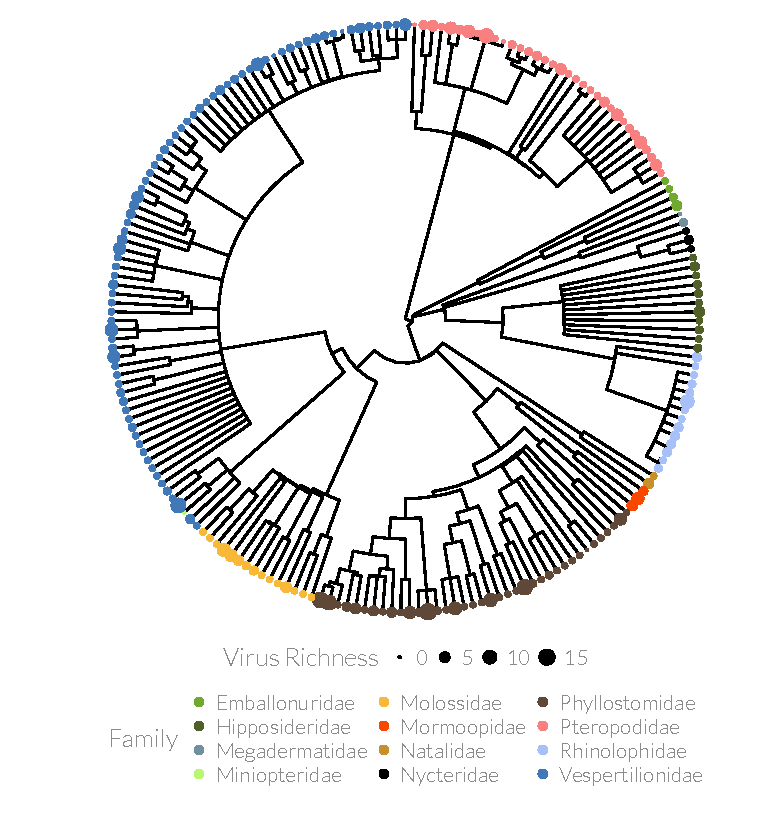
\includegraphics[width=0.8\textwidth]{figure/treePlot-1} 

}

\caption[Pruned phylogeny with dot size showing number of pathogens and colour showing family]{Pruned phylogeny with dot size showing number of pathogens and colour showing family.}\label{fig:treePlot}
\end{figure}


\end{knitrout}



\begin{knitrout}\footnotesize
\definecolor{shadecolor}{rgb}{0.969, 0.969, 0.969}\color{fgcolor}\begin{kframe}


{\ttfamily\noindent\bfseries\color{errorcolor}{\#\# Error in thesis\_colour(): object 'pal' not found}}\end{kframe}
\end{knitrout}



\begin{knitrout}\footnotesize
\definecolor{shadecolor}{rgb}{0.969, 0.969, 0.969}\color{fgcolor}\begin{kframe}


{\ttfamily\noindent\bfseries\color{errorcolor}{\#\# Error in thesis\_colour(): object 'pal' not found}}

{\ttfamily\noindent\bfseries\color{errorcolor}{\#\# Error in thesis\_colour(): object 'pal' not found}}

{\ttfamily\noindent\bfseries\color{errorcolor}{\#\# Error in thesis\_colour(): object 'pal' not found}}

{\ttfamily\noindent\bfseries\color{errorcolor}{\#\# Error in thesis\_colour(): object 'pal' not found}}\end{kframe}
\end{knitrout}




I used two measures of population structure. 
$F_{ST}$ and the number of subspecies.
The number of subspecies was counted using the Wilson and Reeder taxonomy \cite{wilson2005mammal}.
$F_{ST}$ and other measures were collated from the literature.
Studies are from a wide range of spatial scales, from local ($\sim\SI{10}{\kilo\metre}$) to continental.
As $F_{ST}$ inevitably increases with spatial scale I controlled for this by only using data from studies where a large proportion of the species range was studied.
I used the ratio of the furthest distance between $F_{ST}$ samples to the width of the species range and only used studies if this ratio was greater than 0.3.
To allow comparison between different measures ($F_{ST}, \phi_{ST}$) and data from different molecular regions I converted all data to diploid gene flow.
WILL ADD EXTRA METHODS LATER.
These two measures of population structure were analysed separately as the number of subspecies has 196 data points while there is only $F_{ST}$ data for $\sim 30$ bat species.

To control for study bias I collected the number of Pubmed and Google Scholar citations for each bat species including synonyms from ITIS \cite{itis} via the taxize package \cite{chamberlain2013taxize}.
The counts were scraped using the rvest package \cite{rvest}.
I log transformed these variables as they were strongly right skewed.
The log number of citations on Pubmed and Google scholar were highly correlated (pgls: $t$ = 5.58, df = 194, $p$ = \ensuremath{8.04\times 10^{-8}}).
The results here are for analyses using only Google Scholar citations.
See the appendix for analyses run using Pubmed citations.

Measures of body mass are taken from Pantheria \cite{jones2009pantheria}.
They are log transformed due to the strong right skew.



%Pubmed was scraped on pubmedScrapeDate and Google Scholar was scraped on scholarScrapeDate

To control for phylogenetic nonindependance I used the best-supported phylogeny from \cite{fritz2009geographical} which is the supertree from \cite{bininda2007delayed} with names updated to match the Wilson \& Reeder taxonomy \cite{wilson2005mammal}.
Phylogenetic manipulation was performed using the ape package \cite{ape}.


I ran two models using the caper package \cite{caper} testing the relationship between pathogen richness and log number of subspecies.
All independant variables were log transformed.
I ran phylogenetically controlled, multivariate linear models.
This model was fitted both with and without an interaction term between number of subspecies and study effort.

Plots were created with a combination of \cite{ggplot2, palettetown, dotwhisker, ggtree}



%\clearpage







\begin{knitrout}\footnotesize
\definecolor{shadecolor}{rgb}{0.969, 0.969, 0.969}\color{fgcolor}\begin{figure}[t]

{\centering 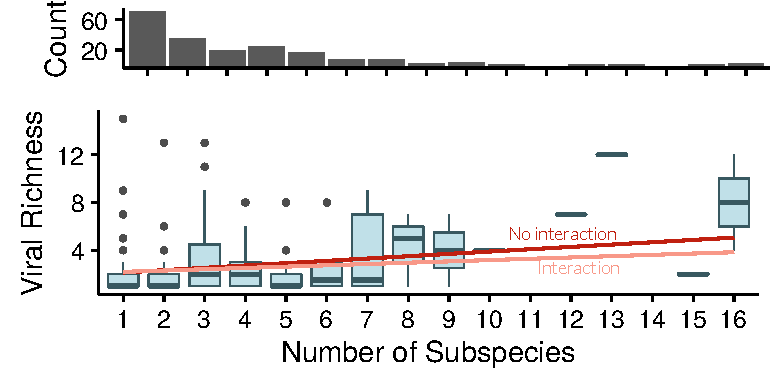
\includegraphics[width=0.8\textwidth]{figure/boxplot-1} 

}

\caption[Number of virus species against number of subspecies]{Number of virus species against number of subspecies. Data within a number of subspecies are plotted as boxplots with the dark bar showing the median, the box showing the interquartile range, vertical lines showing the range and outliers shown as seperate points. A non-phylogenetic linear model is shown in blue}\label{fig:boxplot}
\end{figure}


\end{knitrout}


\begin{knitrout}\footnotesize
\definecolor{shadecolor}{rgb}{0.969, 0.969, 0.969}\color{fgcolor}\begin{kframe}


{\ttfamily\noindent\bfseries\color{errorcolor}{\#\# Error in plot.new(): figure margins too large}}

{\ttfamily\noindent\bfseries\color{errorcolor}{\#\# Error in plot.new(): figure margins too large}}

{\ttfamily\noindent\bfseries\color{errorcolor}{\#\# Error in plot.new(): figure margins too large}}\end{kframe}
\end{knitrout}








\clearpage






\begin{knitrout}\footnotesize
\definecolor{shadecolor}{rgb}{0.969, 0.969, 0.969}\color{fgcolor}\begin{kframe}


{\ttfamily\noindent\bfseries\color{errorcolor}{\#\# Error in thesis\_colour(): object 'pal' not found}}\end{kframe}
\end{knitrout}







\begin{knitrout}\footnotesize
\definecolor{shadecolor}{rgb}{0.969, 0.969, 0.969}\color{fgcolor}\begin{kframe}


{\ttfamily\noindent\bfseries\color{errorcolor}{\#\# Error in thesis\_colour(): object 'pal' not found}}\end{kframe}
\end{knitrout}



%%%%%%%%%%%%%%%%%%%%%%%%%%%%%%%%%%%%%%%%%%%%%%%%%%%%%%%%%%%%%%%%%%%%%%%%%%%%%%%%%%%%%%%%%%%%%%%%%%%%%%%%%%%%%%%%%%%%%%%%%%%%%%%%%%%%%%%%%%%%%%%%%%%%%%%%%%%

\clearpage
\section{Results}

%%%%%%%%%%%%%%%%%%%%%%%%%%%%%%%%%%%%%%%%%%%%%%%%%%%%%%%%%%%%%%%%%%%%%%%%%%%%%%%%%%%%%%%%%%%%%%%%%%%%%%%%%%%%%%%%%%%%%%%%%%%%%%%%%%%%%%%%%%%%%%%%%%%%%%%%%%%


See Figure \ref{fig:plotSubspeciesCoefs} for a display of estimated coefficients for the two models using number of viruses as the response variable. 
The main model with mass, study effort and number of subspecies as predictors found study effort to be highly significant ($\beta = $ NA, $p = $ 0.08). 
The number of subspecies was marginally significant ($\beta = $ 1, $p = $ \ensuremath{8.08\times 10^{-5}}). 
The effect of nonindependance due to phylogeny was very small ($\lambda = $ 0.03, $p = $ 0.44).

The interaction term between study effort and number of subspecies, when included, was not significant ($\beta = $ 0.08, $p = $ 0.64).





\begin{knitrout}\footnotesize
\definecolor{shadecolor}{rgb}{0.969, 0.969, 0.969}\color{fgcolor}\begin{figure}[t]

{\centering 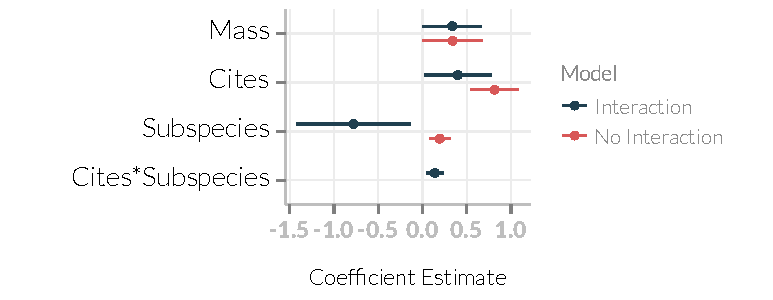
\includegraphics[width=0.8\textwidth]{figure/plotSubspeciesCoefs-1} 

}

\caption[
Plot of coefficient estimates and 95\% confidence intervals for phylogenetic model with (inter) and without (joint) interactions between study effort and number of subspecies]{
Plot of coefficient estimates and 95\% confidence intervals for phylogenetic model with (inter) and without (joint) interactions between study effort and number of subspecies. 
Without interactions, number of subspecies is marginally significant.
}\label{fig:plotSubspeciesCoefs}
\end{figure}


\end{knitrout}


\begin{table}
  \rowcolors{2}{gray!25}{white}
  \begin{tabular}{cc}
  \hline
  Covariate & Estimate ($\pm$ SE) \\
  \hline
  1 &2 \\
  2 & 1 \\



  \end{tabular}
\caption{Table of parameter estimates.}
\label{t:params}
\end{table}







%%%%%%%%%%%%%%%%%%%%%%%%%%%%%%%%%%%%%%%%%%%%%%%%%%%%%%%%%%%%%%%%%%%%%%%%%%%%%%%%%%%%%%%%%%%%%%%%%%%%%%%%%%%%%%%%%%%%%%%%%%%%%%%%%%%%%%%%%%%%%%%%%%%%%%%%%%%

\clearpage
\section{Discussion}  

%%%%%%%%%%%%%%%%%%%%%%%%%%%%%%%%%%%%%%%%%%%%%%%%%%%%%%%%%%%%%%%%%%%%%%%%%%%%%%%%%%%%%%%%%%%%%%%%%%%%%%%%%%%%%%%%%%%%%%%%%%%%%%%%%%%%%%%%%%%%%%%%%%%%%%%%%%%









